% !TeX program = xelatex
\documentclass[12pt,a4paper]{ctexart}
\usepackage{amsfonts,amsmath,amsthm,amssymb,graphicx,url}
\usepackage{fullpage}
\usepackage{enumitem}
\usepackage{tikz}
\usetikzlibrary{arrows.meta, intersections, automata, shapes, positioning, calc}
\allowdisplaybreaks
\setlist[enumerate]{font=\bfseries}


% Old Stuff
%%\oddsidemargin=0.15in
%%\evensidemargin=0.15in
%%\topmargin=-.5in
%%\textheight=9in
%%\textwidth=6.25in

\setlength{\oddsidemargin}{.1in}
\setlength{\evensidemargin}{.1in}
\setlength{\topmargin}{-0.4in}

\newcommand{\heading}[5]{
   \renewcommand{\thepage}{\arabic{page}}
   \noindent
   \begin{center}
   \framebox{
      \vbox{
    \hbox to 6.2in { {\bf B62005Y-02 理论计算机科学基础}
     	 \hfill #2 }
       \vspace{4mm}
       \hbox to 6.2in { {\Large \hfill #5  \hfill} }
       \vspace{2mm}
       \hbox to 6.2in { {\it #3 \hfill #4} }
      }
   }
   \end{center}
   \vspace*{4mm}
}
	
\newcommand{\handout}[3]{\heading{#1}{#2}{主讲教师:杨光}{张远航 \textsc{2015K8009929045}}{#3}}

\setlength{\parindent}{0in}
\setlength{\parskip}{0.1in}

\def\eps{\varepsilon}
\def\a{\texttt{a}}
\def\b{\texttt{b}}
\def\c{\texttt{c}}

\def\der{\Rightarrow}

\begin{document}
\handout{2}{2017年3月29日}{Solutions to Homework \# 2}

\begin{enumerate}
\item[Sipser 2.1](c) Derivations: $E\der E+T\der E+T+T\der E+T+T\der F+T+T\der\ldots\der \a+\a+\a$.

The parse tree:

\begin{center}
	\begin{tikzpicture}[sibling distance=5em, level distance=2em,
	 					every node/.style = {align=center}]]
	\node {$E$}
		child { node {$E$} 
			child { node {$E$} 
				child { node {$T$} 
					child { node {$F$} 
						child { node {\a} }}}}
			child { node {$+$} }
			child { node {$T$} 
				child { node {$F$} 
					child { node {\a} }}}
			}
		child { node {$+$} }
		child { node {$T$} 
			child { node {$F$} 
				child { node {\a} }
		}};
	\end{tikzpicture}
\end{center}

\item[Sipser 2.2](a) First, we show that both $A$ and $B$ are \textsf{CFL}s. The following grammars derive them:
\begin{align*}
S & \to RT\\
R & \to \a R \mid \eps\\
T & \to \b T \c \mid \eps
\end{align*}
and
\begin{align*}
S & \to TR\\
R & \to \a T \b \mid \eps\\
T & \to \c R \mid \eps
\end{align*}
Note that $A\cap B = \{\a^n\b^n\c^n \mid n\ge 0\}$ is not context-free by Example 2.20. We have found a counterexample and therefore the \textsf{CFL}s are not closed under intersection.

(b) \emph{Proof.} We prove this in two parts: 
\begin{itemize}
	\item \emph{\textsf{CFL}s are closed under the union operation.} Let $G_1 = (V_1, \Sigma, R_1, S_1)$ and $G_2 = (V_2, \Sigma, R_2, S_2)$ be two arbitrary \textsf{CFG}s. We can construct a grammar $G = (V, \Sigma , R, S)$ that recognized their union:let $V = V_1\cup V_2$ and $R = R_1\cup R_2\cup \{S\to S_1, S\to S_2\}$. (W.L.O.G. assume that $R_1\cap R_2 = \emptyset$; otherwise rename the variables.)
	\item \emph{\textsf{CFG}s are not closed under complementation.} Assume to the contrary that the \textsf{CFG}s are closed under complementation; then for two \textsf{CFG}s $G_1$ and $G_2$, $\overline{L(G_1)}$ and $\overline{L(G_2)}$ are context-free. It follows that $\overline{L(G_1)}\cup \overline{L(G_2)}$ is context free. Our assumption implies that $\overline{\overline{L(G_1)}\cup \overline{L(G_2)}} = L(G_1)\cap L(G_2)$ (by de Morgan's Law) is also context-free; however, following part (a) and setting $G_1 = A$ and $G_2 = B$ leads us to a contradiction. Therefore the context-free languages are not closed under complementation.\hfill\qed
\end{itemize}
\item[Sipser 2.4](b) The following grammar generates it: 
\begin{align*}
S & \to \mathtt{0}T\mathtt{0}\mid \mathtt{1}T\mathtt{1}
\\T & \to \mathtt{0}T\mathtt{0}\mid \mathtt{1}T \mid \eps
\end{align*}
\item[Sipser 2.6](b) We can write the complement of the language $\{\a^n\b^n\mid n\ge 0\}$ as the union of two languages:
\begin{itemize}
	\item $\{\a^i\b^j\mid i, j\ge 0 , i\ne j\}$, and
	\item arbitrary strings of \a{} and \b{} with ``\b\a" in between: $(\a\cup\b)^*\b\a(\a\cup\b)^*$.
\end{itemize}
The \textsf{CFG}s for them are
\begin{align*}
S_1 & \to \a S_1\b\mid A\mid B\\
A & \to \a A\mid \a\\
B & \to B\b \mid \b
\end{align*}
and
\begin{align*}
S_2 & \to E\b\a E\\
E & \to EE\mid a\mid b\mid\eps
\end{align*}
Combining them we get a \textsf{CFG} for the language asked:
\begin{align*}
S & \to S_1\mid S_2\\
S_1 & \to \a S_1\b\mid A\mid B\\
A & \to \a A\mid \a\\
B & \to B\b \mid \b\\
S_2 & \to E\b\a E\\
E & \to EE\mid a\mid b\mid\eps
\end{align*}
\item[Sipser 2.11]
Here is the constructed automata:
\begin{center}
	\begin{tikzpicture}
	[
	state/.style = {circle, draw, inner sep = 0cm, minimum size = 10pt},
	tip/.style = {
		->,
		>={Stealth[width=6pt,length=9pt]}
	},
	rtip/.style = {
		<-,
		>={Stealth[width=6pt,length=9pt]}
	}
	]
	
	\node[state,ellipse, inner sep = 3pt, initial, initial text = ] (qstart) {$q_\mathrm{start}$};
	\node[state, below = of qstart] (qbuf) {};
	\node[state,ellipse, inner sep = 3pt, below = of qbuf] (qloop) {$q_\mathrm{loop}$};
	\node[state,ellipse, inner sep = 3pt, accepting, below = of qloop] (qacc) {$q_\mathrm{accept}$};
	\node[state, above right = 2cm and 4cm of qloop](ll){};
	\node[state, right = 2cm of ll] (lr) {};
	\node[state, above = of ll] (ml) {};
	\node[state, right = 2cm of ml] (mr) {};
	\node[state, above = of ml] (ul) {};
	\node[state, right = 2cm of ul] (ur) {};
	
	\draw[rtip] (ll) -- node[above] {$\eps$, $F$; )}++(-3, 0) -- (qloop);
	\draw[rtip] (ml) -- node[above] {$\eps$, $T$; $F$}++(-3, 0) -- (qloop);
	\draw[rtip] (ul) -- node[above] {$\eps$, $E$; $T$}++(-3, 0) -- (qloop);
	\draw[tip] (ll) -- node[above] {$\eps$, $\eps$; $E$}++(lr);
	\draw[tip] (ml) -- node[above] {$\eps$, $\eps$; $\times$}++(mr);
	\draw[tip] (ul) -- node[above] {$\eps$, $\eps$; +}++(ur);
	\draw[tip] (ur) -| node[pos=.25, above] {$\eps$, $\eps$; $E$} ($(qloop.east -| lr.east)+(4, 1.5)$) coordinate (c0) -- (qloop.east);
	\draw[tip] (mr) -| node[pos=.25, above] {$\eps$, $\eps$; $T$} ($(c0)!0.1!(qloop.east)$);
	\draw[tip] (lr) -| node[pos=.25, above] {$\eps$, $\eps$; (} ($(c0)!0.2!(qloop.east)$);
	\draw[tip] (qstart) -- node[left] {$\eps$, $\eps$; \$}++(qbuf);
	\draw[tip] (qbuf) -- node[left] {$\eps$, $\eps$; $E$}++(qloop);
	\draw[tip] (qloop) -- node[left] {$\eps$, \$; $\eps$}++(qacc);
	\path[->] (qloop) edge[loop left] node[align=center]{\a, \a; $\eps$\\ +, +; $\eps$\\ (, (; $\eps$\\ ), ); $\eps$\\ $\times$, $\times$; $\eps$\\ $\eps$, $F$; \a\\ $\eps$, $E$; $T$\\ $\eps$, $T$; $F$}(2);
	\end{tikzpicture}
\end{center}

\item[Sipser 2.14]
First, add a start variable:
\begin{align*}
S & \to A\\
A & \to BAB\mid B\mid \eps\\
B & \to \mathtt{00}\mid\eps
\end{align*}
Second, remove all $\eps$-rules. We remove $B\to\eps$:
\begin{align*}
S & \to A\\
A & \to BAB\mid B\mid AB\mid BA\mid A\mid\eps\\
B & \to \mathtt{00}
\end{align*}
Also remove $A\to\eps$:
\begin{align*}
S & \to A\mid\eps\\
A & \to BAB\mid B\mid AB\mid BA\mid BB\mid A\\
B & \to \mathtt{00}
\end{align*}
Third, we handle all unit rules. Remove $A\to A$:
\begin{align*}
S & \to BAB\mid B\mid AB\mid BA\mid BB\mid \eps\\
A & \to BAB\mid B\mid AB\mid BA\mid BB\\
B & \to \mathtt{00}
\end{align*}
Also remove $A\to B$:
\begin{align*}
S & \to BAB\mid B\mid AB\mid BA\mid BB\mid \mathtt{00}\mid\eps\\
A & \to BAB\mid B\mid AB\mid BA\mid BB\mid \mathtt{00}\\
B & \to \mathtt{00}
\end{align*}
Finally, convert it into Chomsky normal form:
\begin{align*}
S & \to BC\mid AB\mid BA\mid BB\mid UU\mid \eps\\
A & \to BC\mid AB\mid BA\mid BB\mid UU\\
C & \to AB\\
B & \to UU\\
U & \to \mathtt{0}
\end{align*}
\end{enumerate}
\end{document}
